%!TEX root = ../rapport.tex
\chapter{Conception de l'application générale}
Dans ce chapitre, la conception de l'application générale est exposée. Celle-ci n'est pas des plus détaillée car une conception plus spécifique du client et du serveur se feront respectivement dans les parties \ref{section:conception_client} et \ref{section:conception_serveur}.

\section{Diagramme de cas d'utilisation} % (fold)
\label{sec:diagramme_de_cas_d_utilisation}

La première étape de cette conception a été d'exprimer, simplement, ce qui sera possible de faire dans l'application et d'avoir une base pour en discuter avec un client. Pour se faire, un diagramme des cas d'utilisation a été dessiné et est représenté par la figure \ref{gra:usecase}. Par la suite, une explication des différents éléments importants à la compréhension de ce diagramme est présentée.

\begin{figure}[H]
    	\centering
    	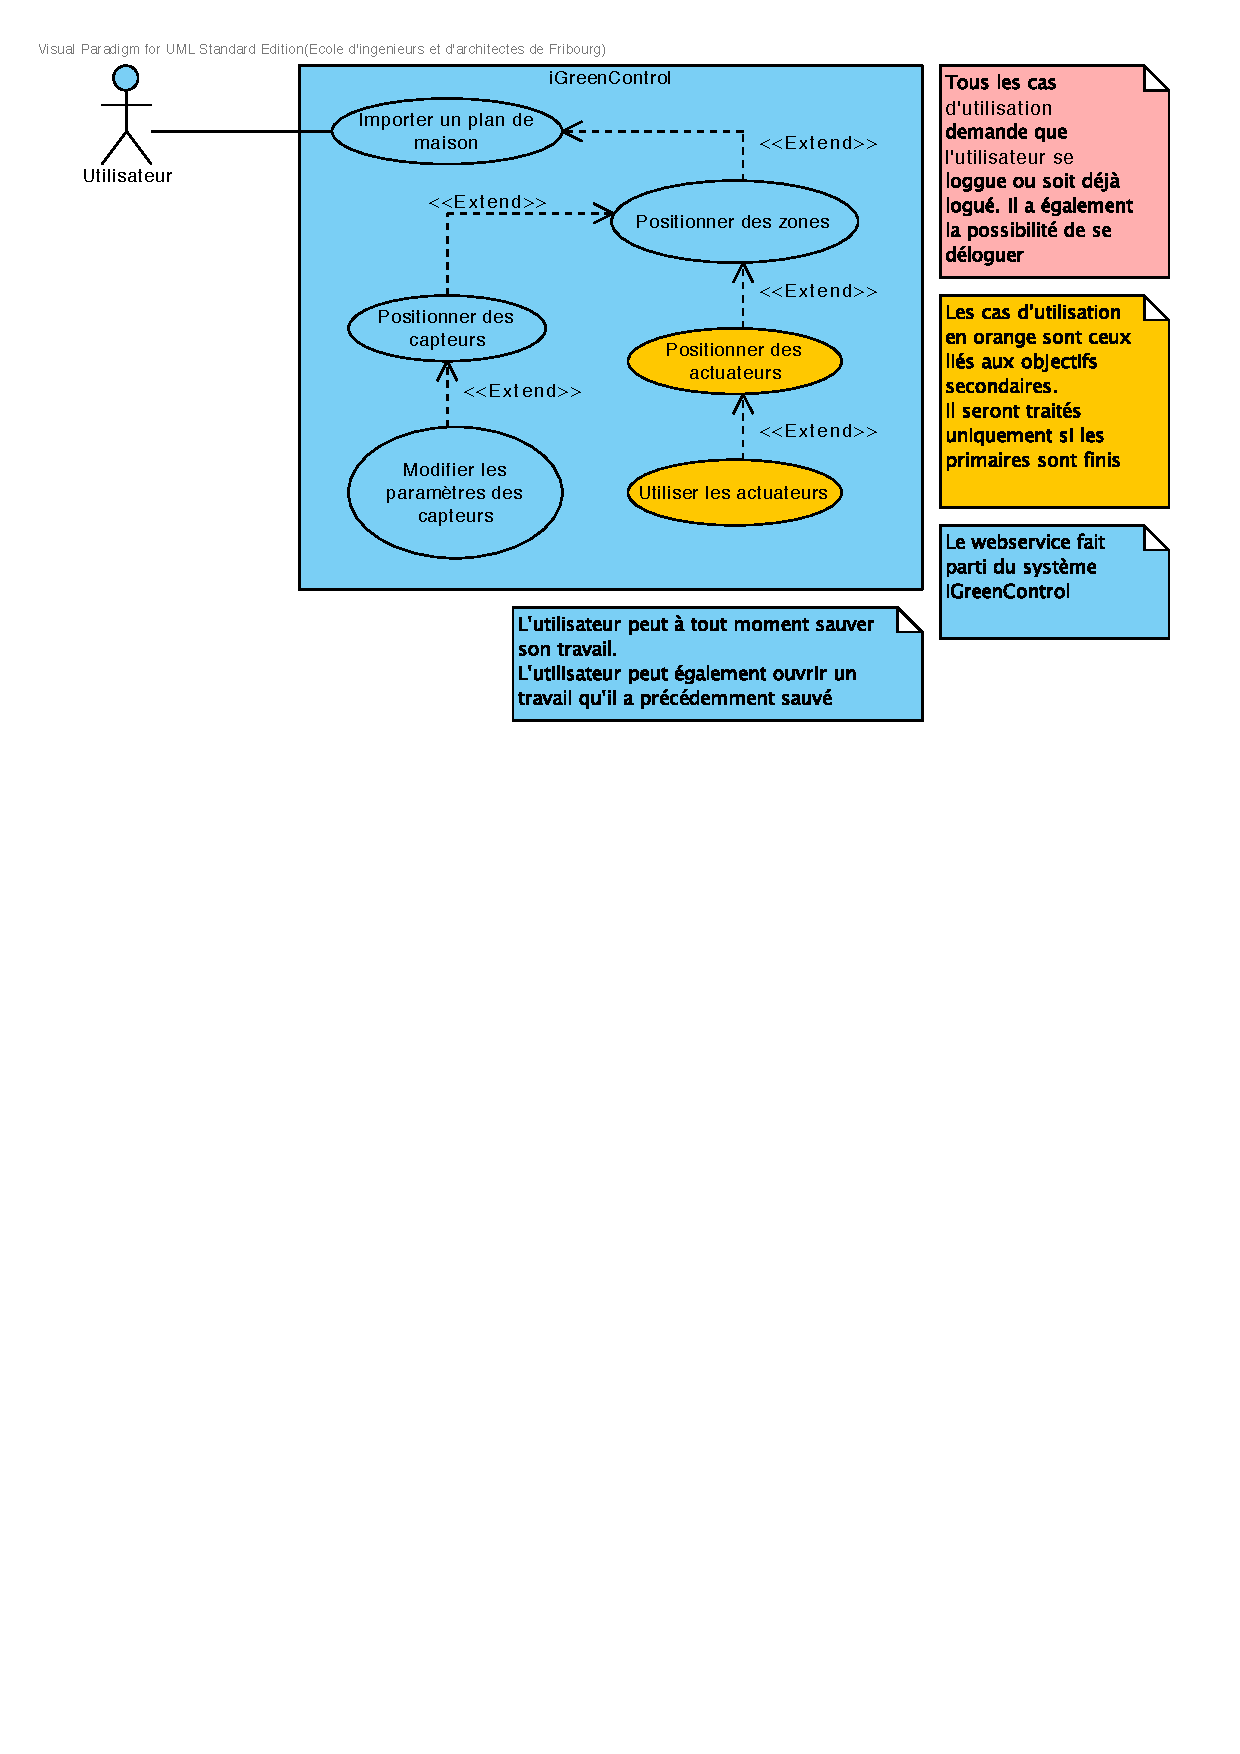
\includegraphics[width=\textwidth]{00_media/04_diagramme_usecase.pdf}
    	\caption{Diagramme de cas d'utilisation du système iGreenControl}
    	\label{gra:usecase}
\end{figure}


\subsection{Les cas d'utilisation} % (fold)

Ci-dessous une explication des différents cas d'utilisation. Ces explications sont brèves car elles seront repris plus en détails dans la partie \ref{section:conception_client}.

\medskip

\begin{itemize}
	\item \textbf{Importer un  plan de maison} consiste à permettre à l'utilisateur final de choisir par exemple une photo dans la librairie des photos et de l'importer dans l'application. 
	\item \textbf{Positionner des zones} demande que l'utilisateur ait importé un plan. Il peut ainsi disposer différentes zones sur ce plan.
	\item \textbf{Positionner des capteurs} demande que l'utilisateur ait positionné des zones sur le plan. Il peut ainsi insérer des capteurs.
	\item \textbf{Modifier les paramètres des capteurs} demande que l'utilisateur ait positionné des capteurs dans des zones. Il peut ainsi en modifier différentes paramètres (nom, catégorie, ...)
	\item \textbf{Positionner des actuateurs} demande que l'utilisateur ait positionné des zones sur le plan. Il peut ainsi insérer des actuateurs. Ceci est un cas d'utilisation issu d'un objectif secondaire.
	\item \textbf{Utiliser les actuateurs} demande que l'utilisateur ait inséré des actuateurs dans des zones. Il peut ainsi utiliser les actuateurs. Ceci est un cas d'utilisation issu d'un objectif secondaire.
\end{itemize}

\subsection{Utilisateur}

L'acteur principal de ce système est l'utilisateur final qui se servira de l'\emph{\gls{ipad}} pour utiliser l'application \emph{iGreenControl}.

\subsection{Authentification}
Sur le diagramme, le fait de devoir s'identifier à l'aide d'un nom d'utilisateur et d'un mot de passe n'a pas été reporté en tant que cas d'utilisation mais en tant que note. Cela a été fait pour alléger le diagramme. 

\begin{shadequote}
Tous les cas d'utilisation demande que l'utilisateur se loggue ou soit déjà logué. Il a également la possibilité de se déloguer. \par\emph{Note du cas d'utilisation}
\end{shadequote}

\subsection{Ouverture et sauvegarde}
Sur le diagramme, le fait de pouvoir sauvegarder et ouvrir un travail n'est pas représenter et est introduit par une note. Cela a été fait pour alléger le diagramme.

\begin{shadequote}
L'utilisateur peut à tout moment sauver son travail.
L'utilisateur peut également ouvrir un travail qu'il a précédemment sauvé. \par\emph{Note du cas d'utilisation}
\end{shadequote}


\subsection{Webservice}

Le tout s'articulera autour d'un \emph{\gls{webservice}} qui permettra de demander et d'envoyer des informations dans la base de données. Comme ce service fait parti du système, il  n'est pas représenté par un acteur mais est bel et bien dans le système \emph{iGreenControl}.

\begin{shadequote}
Le \emph{\gls{webservice}} fait parti du système iGreenControl. \par\emph{Note du cas d'utilisation}
\end{shadequote}


\subsection{Objectifs primaires et secondaires}
Le diagramme différencie les objectifs primaires des objectifs secondaires.

\begin{shadequote}
Les cas d'utilisation en orange sont ceux liés aux objectifs secondaires.
Il seront traités uniquement si les primaires sont finis. \par\emph{Note du cas d'utilisation}
\end{shadequote}

% subsection explications (end)

% section diagramme_de_cas_d_utilisation (end)
\section{Scénario générale de l'application} % (fold)
\label{sub:concept_de_l_application}
L'utilisateur importe une photo du plan de sa maison ou son appartement. 

\medskip

Il peut ensuite créer des zones par pièce (ex: une chambre = une zone). Les pièces du même type peuvent être regroupées dans une zone (ex: toutes les chambres = une zone "mère").

\medskip

Lorsque ceci est fait, il a la possibilité de positionner des capteurs dans les différentes zones et gérer les paramètres généraux de ceux-ci.

\medskip

Enfin, les données récupérées pourront être exploitées par d'autres personnes en vue de faire de l'économie d'énergie. Ce projet a donc un principe d'informatique écologique. 

\medskip

Optionnellement, des actuateurs pourront être placés dans des zones dans le but par exemple d'éteindre ou d'allumer une lampe.

% section concept_de_l_application (end)

\section{Architecture générale de l'application} % (fold)
\label{sub:architecture_g_n_rale_de_l_application}
La figure \ref{gra:archiGenerale} représente l'architecture générale de l'application.
\begin{figure}[H]
    	\centering
    	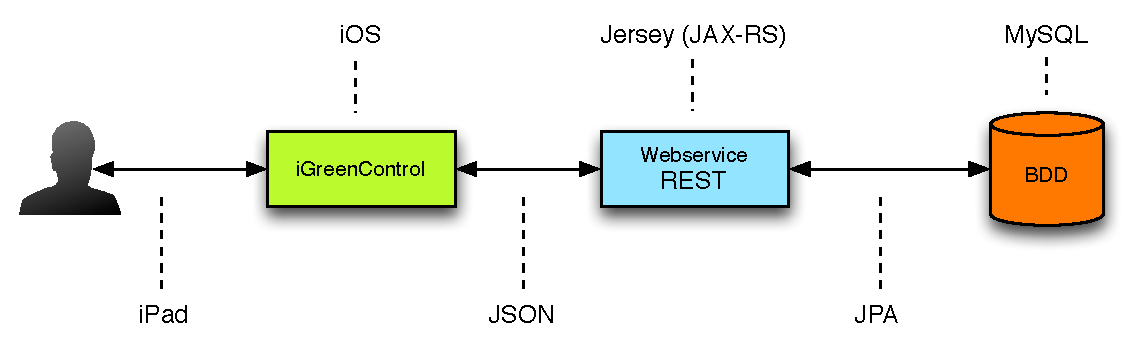
\includegraphics[width=\textwidth]{00_media/02_archi.pdf}
    	\caption{Architecture générale de l'application}
    	\label{gra:archiGenerale}
\end{figure}
% section architecture_g_n_rale_de_l_application (end)


L'utilisateur, muni d'un \emph{\gls{ipad}}, utilise l'application \emph{iGreenControl} qui tourne sur \emph{\gls{ios}}.

\medskip

L'application récupère les données dont elle a besoin sous format \emph{\gls{json}} depuis un \emph{\gls{webservice}}.

\medskip

Le \emph{\gls{webservice}} est de type \emph{\gls{rest}} et implémente \emph{\gls{jaxrs}} qui est une interface de programmation \emph{\gls{java}} qui permet de créer des \emph{\glspl{webservice}}. J'utiliserai \emph{Jersey} qui est une des références en implémentation de \emph{\gls{jaxrs}}.

\medskip

Le \emph{\gls{webservice}} travaille avec une base de données de type \emph{\gls{mysql}} via \emph{\gls{jpa}} qui est une interface de programmation qui permet d'organiser nos données relationnelles avec \emph{\gls{java}}.

\section{Base de données} % (fold)
\label{sec:base_de_donn_es}
Pour ce qui est de la base de données, il n'y a pas eu de grands changements pour le projet si ce n'est ajouter des informations pour retenir :

\medskip

\begin{itemize}
    \item L'image du plan
    \item La position en x et en y du plan
    \item La largeur et la longueur du plan
    \item La position en x et en y d'une zone
    \item La largeur et la longueur d'une zone
    \item La valeur total des rotations effectuée sur une zone
\end{itemize}

\medskip

Le tout a été ajouté sous forme de chaîne de caractères.
% section base_de_donn_es (end)
